
%%%%%%%%%%%%%%%%%%%%%%%%%%%%%%%%%%%%%%%%%%%%%%%%%%%%%%%%%%%%%%%%%%%%%%%%%%%%%%
% Copyright (c) 2003-2014 by University of Queensland
% http://www.uq.edu.au
%
% Primary Business: Queensland, Australia
% Licensed under the Open Software License version 3.0
% http://www.opensource.org/licenses/osl-3.0.php
%
% Development until 2012 by Earth Systems Science Computational Center (ESSCC)
% Development 2012-2013 by School of Earth Sciences
% Development from 2014 by Centre for Geoscience Computing (GeoComp)
%
%%%%%%%%%%%%%%%%%%%%%%%%%%%%%%%%%%%%%%%%%%%%%%%%%%%%%%%%%%%%%%%%%%%%%%%%%%%%%%

%!TEX root = user.tex
\chapter{The escript symbolic toolbox}
\label{CHAP:Symbolic}
\section{Introduction}
\escript builds on the existing Sympy~\cite{Sympy} symbolic maths library to
provide a \SYMBOL class with support for \escript Data objects. \SYMBOL objects
act as placeholders for a single mathematical symbol, such as \texttt{x}, or
for arbitrarily complex mathematical expressions such as
\texttt{c*x**4 + alpha*exp(x) - 2*sin(beta * x)}, where \texttt{alpha},
\texttt{beta}, \texttt{c}, and \texttt{x} are also symbols (the symbolic
``atoms" of the expression).
With the help of the \EVALUATOR class, these symbols and expressions can
be evaluated by substituting numeric values and/or \escript \Data objects
for the atoms. Escript's \SYMBOL class has a shape (and thus a rank) as well
as a dimensionality.
Symbols are useful to perform mathematical simplifications, compute
derivatives, take gradients and in the case of \escript describe PDEs.
As an example of how the symbolic toolbox can be used, consider the following
code extract.
\begin{python}
import esys.escript as es
u = es.Symbol('u')
p = 2*u**2 + 3*u + 1
p2 = es.sin(u)
p3 = p.diff(u)              # p3 = derivative of p with respect to u
evalu = es.Evaluator()
evalu.addExpression(p)
evalu.addExpression(p2)
evalu.addExpression(p3)
evalu.subs(u=2*es.symconstants.pi)
evaluated=evalu.evaluate()
print("p3 =", p3)            # The symbols can be printed, this line will print p3.
print(evaluated)
\end{python}
Running this code outputs:\\\texttt{p3 = 4*u + 3\\(1 + 6*pi + 8*pi**2, 0, 3 + 8*pi)}.\\
To get the numeric value of the expression we replace \texttt{evalu.evaluate()}
with \texttt{evalu.evaluate(evalf=True)}. This results in
\texttt{(98.806, 0, 28.132)}.
The use of these Symbols becomes more interesting in the context of escript
when they are integrated with escript \Data objects.

\section{NonlinearPDE}
The \NLPDE class in escript makes use of the escript \SYMBOL class and allows
for the solution of PDEs of the form:
\begin{equation}
-X_{ij,j} + Y_i = 0
\label{symbolic eq1}
\end{equation}
where $X$ and $Y$ are both functions of $u_{k,j}$ and $u_k$, and $u$ is the
unknown function implemented as a \SYMBOL. $\nabla\cdotp x$ denotes divergence
of $x$.
The \NLPDE class uses the \SYMBOL class to solve the nonlinear PDE given in
\eqn{symbolic eq1}.
The class incorporates Newton's method to find the zeroes of the left hand side
of \eqn{symbolic eq1} and as a consequence finding the $X$ and $Y$ which
satisfy \eqn{symbolic eq1}. 
Consecutive updates are calculated until the equation is satisfied to the
desired level of accuracy. The solution to each update step involves solving a
linear PDE. The \NLPDE class uses $X$ and $Y$ to produce the coefficients of
the linear PDE for the update step. The linear PDE class given in
\Sec{SEC LinearPDE} is used to solve the linear PDEs from the update step.
The coefficients of the linear PDE to be solved are calculated as follows: 
\begin{equation*}
 A_{ijkl} = \frac{\partial \text{X}_{ij}}{\partial u_{k,l}}, B_{ijkl} = \frac{\partial \text{X}_{ij}}{\partial u_{k}}, C_{ijkl} = \frac{\partial \text{Y}_{ij}}{\partial u_{k,l}}, D_{ijkl} = \frac{\partial \text{Y}}{\partial u_{k}}
\end{equation*}
\section{2D Plane Strain Problem}
The \NLPDE class can be used to solve a 2D plane strain problem. In continuous
media, stress is given by Lam\'e's \eqn{symbolic eq2}.
\begin{equation} 
-\sigma_{ij,j}=f
\label{symbolic eq2}
\end{equation} 
Hook's Law provides a relation between $\sigma$ and $\epsilon$ in the following form
\begin{equation}
\left[ \begin{array}{c}
\sigma_{00} \\
\sigma_{11} \\
\sigma_{01} \\
\end{array} \right] = 
\left[ \begin{array}{ccc}
c_{00} & c_{01} & c_{05}\\
c_{01} & c_{11} & c_{15}\\
c_{05} & c_{15} & c_{55}\\
\end{array}\right]
\left[ \begin{array}{c}
\epsilon_{00} \\
\epsilon_{11} \\
2\epsilon_{10} \\
\end{array} \right]
\label{symbolic eq3}
\end{equation}
Where $\epsilon = symmetric(grad(u)) \text{ or } %
\epsilon_{ij}=\frac{1}{2}\left(\frac{\partial u_i}{\partial x_j} + %
{\frac{\partial u_j}{\partial x_i}}\right)$, $u$ is the unknown function and
$c_{ij}$ is the stiffness matrix. To fit this to the nonlinear PDE class'
standard form, X is set to $C \times symmetric(grad(u))$.
The following \PYTHON extract shows how an example 2D plane strain problem can
be set up. 

\begin{python}
from esys.escript import *
from esys.finley import Rectangle
#set up domain and symbols
mydomain = Rectangle(l0=1.,l1=1.,n0=10, n1=10)
u = Symbol('u',(2,), dim=2)
q = Symbol('q', (2,2))
sigma = Symbol('sigma',(2,2))
theta = Symbol('theta')
# q is a rotation matrix represented by a Symbol. Values can be substituted for 
# theta.
q[0,0]=cos(theta)
q[0,1]=-sin(theta)
q[1,0]=sin(theta)
q[1,1]=cos(theta)
# Theta gets substituted by pi/4 and masked to lie between .3 and .7 in the 
# vertical direction. Using this masking means that when q is used it will apply
# only to the specified area of the domain. 
x = Function(mydomain).getX()
q=q.subs(theta,(symconstants.pi/4)*whereNonNegative(x[1]-.30)*whereNegative(x[1]-.70))
# epsilon is defined in terms of u and has the rotation applied. 
epsilon0 = symmetric(grad(u))
epsilon = matrixmult(matrixmult(q,epsilon0),q.transpose(1))
# For the purposes of demonstration, an arbitrary c with isotropic constraints 
# is chosen here. In order to act as an isotropic material c is chosen such that 
# c00 = c11 = c01+c1+2*c55
c00 = 10
c01 = 8; c11 = 10
c05 = 0; c15 = 0; c55 = 1
# sigma is defined in terms of epsilon
sigma[0,0] = c00*epsilon[0,0]+c01*epsilon[1,1]+c05*2*epsilon[1,0]
sigma[1,1] = c01*epsilon[0,0]+c11*epsilon[1,1]+c15*2*epsilon[1,0]
sigma[0,1] = c05*epsilon[0,0]+c15*epsilon[1,1]+c55*2*epsilon[1,0]
sigma[1,0] = sigma[0,1]
sigma0=matrixmult(matrixmult(q.transpose(1),sigma),q)
# set up boundary conditions
x=mydomain.getX()
gammaD=whereZero(x[1])*[1,1]
yconstraint = FunctionOnBoundary(mydomain).getX()[1]
# The nonlinear PDE is set up, the values are substituted in and the solution is
# calculated, y represents an external shearing force acting on the domain. 
# In this case a force of magnitude 50 is acting in the x[0] direction.
p = NonlinearPDE(mydomain, u, debug=NonlinearPDE.DEBUG0)
p.setValue(X=sigma0,q=gammaD,y=[-50,0]*whereZero(yconstraint-1),r=[1,1])
v = p.getSolution(u=[0,0])
\end{python}
%\pagebreak
The way in which the rotation matrix q is set up demonstrates the seamless integration of escript symbols and \Data objects. A \SYMBOL is used to set up the matrix, the values for theta are then later substituted in. The example also demonstrates how the symbolic toolbox can be used as an aid to easily move from a mathematical equation to an escript data object which can be used to do numerical calculations. 
Running the script calculates the unknown function u and assigns it to v. We can use v to calculate the stress and strain.  
\begin{table}[!h]
\centering
\begin{tabular}{|c|c|c|}
  \hline
   & Anisotropic & Isotropic\\%\multicolumn{2}{|c|}{Isotopic} \\
  \hline
  No rotation & 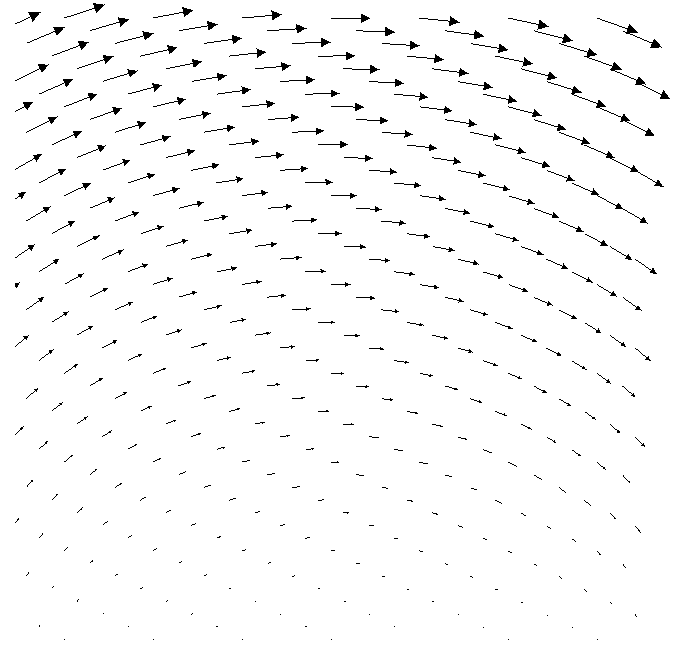
\includegraphics[scale=0.2]{0RotAniso} & 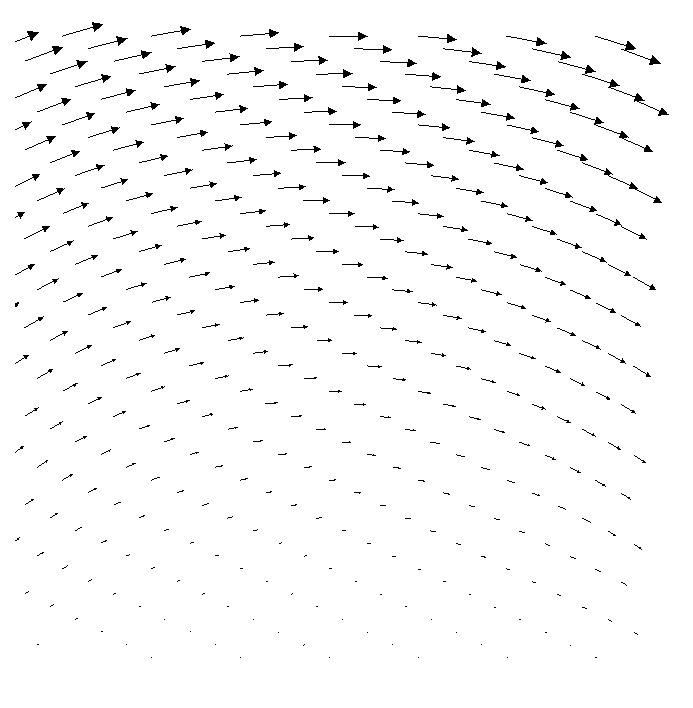
\includegraphics[scale=0.2]{0RotIso}\\
  \hline
  60\textdegree\ rotation & 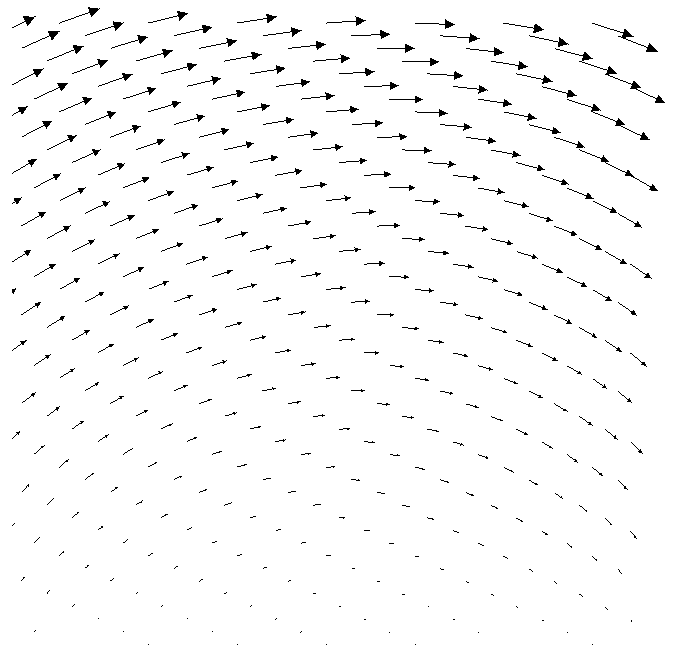
\includegraphics[scale=0.2]{MidRotAniso} & 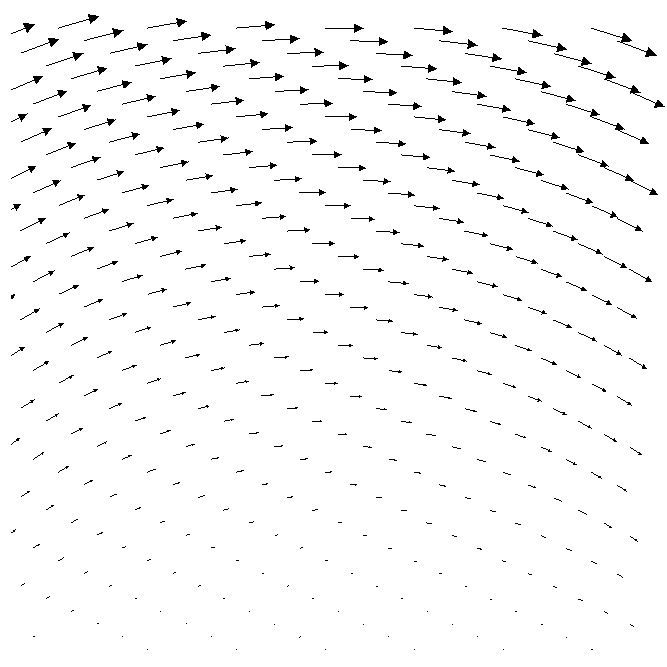
\includegraphics[scale=0.2]{MidRotIso}\\ 
  \hline
  difference & 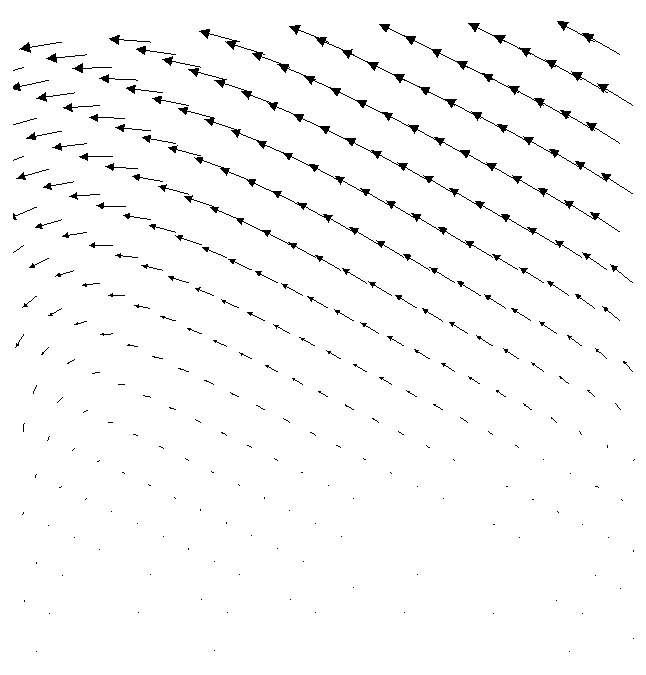
\includegraphics[scale=0.2]{diffaniso} & \raisebox{2cm}{no difference}\\ 
  \hline
\end{tabular}
\caption{Displacement vectors calculated using \NLPDE}
\label{isovsaniso}
\end{table}
Table \ref{isovsaniso}, shows the result of running the above script under varying values of c and theta. Both isotropic and anisotropic cases are considered.  For the anisotropic case, $c_{ij}$ is chosen such that
$c00 = c11 = c01+c1+2*c55$ does not hold.
Two values of theta are also considered; one with a masked 60\textdegree
rotation in the middle and one with no rotation.
The last row of the table shows the difference between rotation in the middle
and no rotation. In the isotropic case it can be seen that there is no
difference in the output when the rotation is applied.
There is however, an obvious difference when the anisotropic case is considered.

\section{Classes}
A number of classes are associated with escript symbols. A detailed listing of the definitions and usage is provided below. 
\subsection{Symbol class}
\begin{classdesc}{Symbol}{symbol \optional{, shape} \optional{, Dim}}
Defines a \SYMBOL object. The first argument \member{symbol} is a string given
to represent the \SYMBOL. The string typically matches the name of the object,
for instance \texttt{u=Symbol('u')}. Next optional \member{shape} argument
defines whether the \SYMBOL is a scalar, vector, matrix, or tensor and the
length or size of it. \member{dim} is used to define the dimensionality of the
object contained in the \SYMBOL.
For a \SYMBOL definition \texttt{u = Symbol('u',(10,), dim=2)}, the value of u
will be a vector with 10 components and the domain on which u will be used is
2-dimensional (this is relevant with operations such as \texttt{grad} where the
number of spatial dimensions is important). 
\end{classdesc}
\subsubsection{Symbol class methods}
\begin{methoddesc}[Symbol]{atoms}{\optional{types}}
Returns the atoms that form the current \SYMBOL.
By default, only objects that are truly atomic and cannot be divided into
smaller pieces are returned: symbols, numbers, and number symbols like $e$ and
$pi$. It is possible to request atoms of any type via the \member{types}
argument, however.
\end{methoddesc}

\begin{methoddesc}[Symbol]{coeff}{x \optional{, expand=true}}
Returns the coefficient of the term \texttt{x} or $0$ if there is no \texttt{x}.
If \texttt{x} is a scalar \SYMBOL then \texttt{x} is searched in all components
of this \SYMBOL. Otherwise the shapes must match and the coefficients are
checked component by component. For example:
\begin{python}
     x=Symbol('x', (2,2))
     y=3*x
     print y.coeff(x)
     print y.coeff(x[1,1])
\end{python}
will print:
\begin{python}
     [[3 3]
      [3 3]]
     [[0 0]
      [0 3]]
\end{python} 
\end{methoddesc}
\begin{methoddesc}[Symbol]{diff}{symbols}
Takes the derivative of the \SYMBOL object of which the method is called with
respect to the symbols specified in the argument \member{symbols}.
\end{methoddesc}
\begin{methoddesc}[Symbol]{evalf}{}
Applies the \texttt{sympy.evalf} operation on all elements of the \SYMBOL which
are of type or inherit from \texttt{sympy.Basic}.
\end{methoddesc}
\begin{methoddesc}[Symbol]{expand}{}
Applies the \texttt{sympy.expand} operation on all elements in this \SYMBOL.
\end{methoddesc}
%\begin{methoddesc}[Symbol]{getDataSubstitutions}{}
%end{methoddesc}
\begin{methoddesc}[Symbol]{getDim}{}
Returns the \SYMBOL's spatial dimensionality, or -1 if undefined.
\end{methoddesc}
\begin{methoddesc}[Symbol]{getRank}{}
Returns the \SYMBOL's rank which is equal to the length of the shape.
\end{methoddesc}
\begin{methoddesc}[Symbol]{getShape}{}
Returns the shape of this \SYMBOL.
\end{methoddesc}
\begin{methoddesc}[Symbol]{grad}{\optional{where=none}}
Returns the gradient of this \SYMBOL. The \SYMBOL must have a dimensionality
defined in order for \texttt{grad} to work. As with the normal escript
\texttt{grad} function a \FunctionSpace can be specified using the
\member{where} argument. The \FunctionSpace should be wrapped in a \SYMBOL.
To do this, set up a \SYMBOL and then use the \texttt{subs} function to
substitute in the \FunctionSpace.
\end{methoddesc}
\begin{methoddesc}[Symbol]{inverse}{}
Find the inverse of the \SYMBOL to which the function is applied. Inverse is only valid for square rank 2 symbols.
\end{methoddesc}
%\begin{methoddesc}[Symbol]{item}{}
%\end{methoddesc} 
%\begin{methoddesc}[Symbol]{lambdarepr}{}
%test
%\end{methoddesc}
\begin{methoddesc}[Symbol]{simplify}{}
Applies the \texttt{sympy.simplify} operation on all elements in this \SYMBOL.
\end{methoddesc}
\begin{methoddesc}[Symbol]{subs}{old, new}
Substitutes or replaces a \SYMBOL specified in \member{old} with whatever is in
\member{new} for this \SYMBOL. Consider:
  \begin{python}
     import esys.escript as es
     u=es.Symbol("u")
     expr=2*u
     expr.subs(u,2)
\end{python}
This prints 4.
\end{methoddesc}
\begin{methoddesc}[Symbol]{trace}{axis_offset}
Returns the trace of the \SYMBOL object.
\end{methoddesc}

\subsection{Evaluator class}
The \EVALUATOR class is intended to have a group of expressions added to it,
substitutions can be made across all expressions and the expressions can then
all be evaluated.
\subsubsection{Evaluator class methods}
\begin{classdesc}{Evaluator}{\optional{expressions}}
An \EVALUATOR object is initiated via \texttt{Evaluator()} with an optional
argument of expressions to store.
\end{classdesc}
\begin{methoddesc}[Evaluator]{addExpression}{expression}
Adds an expression to this \EVALUATOR.
\end{methoddesc}
\begin{methoddesc}[Evaluator]{evaluate}{\optional{evalf=False}\optional{, args}}
Evaluates all expressions in this \EVALUATOR and returns the result as a tuple.
\member{evalf} can be set to \texttt{True} to call \texttt{evalf} on any sympy
symbols which may be part of the expression.
\member{args} can be provided to make any substitutions before the expression
is evaluated.
\end{methoddesc}
\begin{methoddesc}[Evaluator]{subs}{old,new}
Substitutes or replaces a \SYMBOL specified in \member{old} with whatever is
in \member{new} for all expressions in the \EVALUATOR.
\end{methoddesc}

\subsection{NonlinearPDE class}
\begin{classdesc}{NonlinearPDE}{domain, u}
Defines a general nonlinear, steady, second order PDE for an unknown function
\var{u} on a given domain defined through a \Domain object \var{domain}.
\var{u} is a \SYMBOL object.
The general form is -div(X) + Y = 0 
\end{classdesc}
\iffalse
\begin{methoddesc}[NonlinearPDE]{concatenateRow}{}
test
\end{methoddesc}
\begin{methoddesc}[NonlinearPDE]{createCoefficient}{}
test
\end{methoddesc}
\begin{methoddesc}[NonlinearPDE]{getUnknownSymbol}{}
test
\end{methoddesc}
\begin{methoddesc}[NonlinearPDE]{getLinearSolverOptions}{}
test
\end{methoddesc}
\begin{methoddesc}[NonlinearPDE]{getLinearPDE}{}
test
\end{methoddesc}
\begin{methoddesc}[NonlinearPDE]{getNumSolutions}{}
test
\end{methoddesc}
\begin{methoddesc}[NonlinearPDE]{getShapeOfCoefficient}{}
test
\end{methoddesc}
\begin{methoddesc}[NonlinearPDE]{getCoefficient}{}
test
\end{methoddesc}
\begin{methoddesc}[NonlinearPDE]{getSensitivity}{}
test
\end{methoddesc}
\fi
\begin{methoddesc}[NonlinearPDE]{getSolution}{subs}
Returns the solution of the PDE. \member{subs} contatins the substitutions for
all symbols used in the coefficients including the initial value for the
unknown \texttt{u}.
\end{methoddesc}
\begin{methoddesc}[NonlinearPDE]{setOptions}{opts}
\begin{verbatim}
  Allows setting options for the nonlinear PDE.
  The supported options are:
    tolerance
        error tolerance for the Newton method
    iteration_steps_max
        maximum number of Newton iterations
    omega_min
        minimum relaxation factor
    atol
        solution norms less than atol are assumed to be atol.
        This can be useful if one of your solutions is expected to
        be zero.
    quadratic_convergence_limit
        if the norm of the Newton-Raphson correction is reduced by
        less than quadratic_convergence_limit between two iteration
        steps, quadratic convergence is assumed.
    simplified_newton_limit
        if the norm of the defect is reduced by less than
        simplified_newton_limit between two iteration steps and
        quadratic convergence is detected, the iteration switches to the
        simplified Newton-Raphson scheme.
\end{verbatim}

\end{methoddesc}
\begin{methoddesc}[NonlinearPDE]{setValue}{
\optional{X}\optional{, Y}
\optional{, y}
\optional{, q}\optional{, r}}
Assigns new values to coefficients. By default all values are assumed to be
zero\footnote{In fact, it is assumed they are not present by assigning the
value \code{escript.Data()}. This can be used by the solver library to reduce
computational costs.}.
If the new coefficient value is not a \Data object, it is converted into a
\Data object in the appropriate \FunctionSpace.
\end{methoddesc}

\subsection{Symconsts class}
Symconsts provides symbolic constants for use in symbolic expressions. These constants are preferred to floating point implementation as they can cancel perfectly when mathematical expressions are evaluated, avoiding numerical imprecision. 
\begin{verbatim}
usage:
  symconsts.pi this provides a Symbol object

Available constants currently include:
  pi and e 
\end{verbatim}
